\documentclass[twoside]{book}

% Packages required by doxygen
\usepackage{fixltx2e}
\usepackage{calc}
\usepackage{doxygen}
\usepackage[export]{adjustbox} % also loads graphicx
\usepackage{graphicx}
\usepackage[utf8]{inputenc}
\usepackage{makeidx}
\usepackage{multicol}
\usepackage{multirow}
\PassOptionsToPackage{warn}{textcomp}
\usepackage{textcomp}
\usepackage[nointegrals]{wasysym}
\usepackage[table]{xcolor}

% Font selection
\usepackage[T1]{fontenc}
\usepackage[scaled=.90]{helvet}
\usepackage{courier}
\usepackage{amssymb}
\usepackage{sectsty}
\renewcommand{\familydefault}{\sfdefault}
\allsectionsfont{%
  \fontseries{bc}\selectfont%
  \color{darkgray}%
}
\renewcommand{\DoxyLabelFont}{%
  \fontseries{bc}\selectfont%
  \color{darkgray}%
}
\newcommand{\+}{\discretionary{\mbox{\scriptsize$\hookleftarrow$}}{}{}}

% Page & text layout
\usepackage{geometry}
\geometry{%
  a4paper,%
  top=2.5cm,%
  bottom=2.5cm,%
  left=2.5cm,%
  right=2.5cm%
}
\tolerance=750
\hfuzz=15pt
\hbadness=750
\setlength{\emergencystretch}{15pt}
\setlength{\parindent}{0cm}
\setlength{\parskip}{3ex plus 2ex minus 2ex}
\makeatletter
\renewcommand{\paragraph}{%
  \@startsection{paragraph}{4}{0ex}{-1.0ex}{1.0ex}{%
    \normalfont\normalsize\bfseries\SS@parafont%
  }%
}
\renewcommand{\subparagraph}{%
  \@startsection{subparagraph}{5}{0ex}{-1.0ex}{1.0ex}{%
    \normalfont\normalsize\bfseries\SS@subparafont%
  }%
}
\makeatother

% Headers & footers
\usepackage{fancyhdr}
\pagestyle{fancyplain}
\fancyhead[LE]{\fancyplain{}{\bfseries\thepage}}
\fancyhead[CE]{\fancyplain{}{}}
\fancyhead[RE]{\fancyplain{}{\bfseries\leftmark}}
\fancyhead[LO]{\fancyplain{}{\bfseries\rightmark}}
\fancyhead[CO]{\fancyplain{}{}}
\fancyhead[RO]{\fancyplain{}{\bfseries\thepage}}
\fancyfoot[LE]{\fancyplain{}{}}
\fancyfoot[CE]{\fancyplain{}{}}
\fancyfoot[RE]{\fancyplain{}{\bfseries\scriptsize Generated by Doxygen }}
\fancyfoot[LO]{\fancyplain{}{\bfseries\scriptsize Generated by Doxygen }}
\fancyfoot[CO]{\fancyplain{}{}}
\fancyfoot[RO]{\fancyplain{}{}}
\renewcommand{\footrulewidth}{0.4pt}
\renewcommand{\chaptermark}[1]{%
  \markboth{#1}{}%
}
\renewcommand{\sectionmark}[1]{%
  \markright{\thesection\ #1}%
}

% Indices & bibliography
\usepackage{natbib}
\usepackage[titles]{tocloft}
\setcounter{tocdepth}{3}
\setcounter{secnumdepth}{5}
\makeindex

% Hyperlinks (required, but should be loaded last)
\usepackage{ifpdf}
\ifpdf
  \usepackage[pdftex,pagebackref=true]{hyperref}
\else
  \usepackage[ps2pdf,pagebackref=true]{hyperref}
\fi
\hypersetup{%
  colorlinks=true,%
  linkcolor=blue,%
  citecolor=blue,%
  unicode%
}

% Custom commands
\newcommand{\clearemptydoublepage}{%
  \newpage{\pagestyle{empty}\cleardoublepage}%
}

\usepackage{caption}
\captionsetup{labelsep=space,justification=centering,font={bf},singlelinecheck=off,skip=4pt,position=top}

%===== C O N T E N T S =====

\begin{document}

% Titlepage & ToC
\hypersetup{pageanchor=false,
             bookmarksnumbered=true,
             pdfencoding=unicode
            }
\pagenumbering{roman}
\begin{titlepage}
\vspace*{7cm}
\begin{center}%
{\Large Notes }\\
\vspace*{1cm}
{\large Generated by Doxygen 1.8.11}\\
\end{center}
\end{titlepage}
\clearemptydoublepage
\tableofcontents
\clearemptydoublepage
\pagenumbering{arabic}
\hypersetup{pageanchor=true}

%--- Begin generated contents ---
\chapter{Hierarchical Index}
\section{Class Hierarchy}
This inheritance list is sorted roughly, but not completely, alphabetically\+:\begin{DoxyCompactList}
\item \contentsline{section}{About\+Me\+View\+Controller()}{\pageref{category_about_me_view_controller_07_08}}{}
\item $<$U\+I\+Application\+Delegate$>$\begin{DoxyCompactList}
\item \contentsline{section}{V\+T\+K\+App\+Delegate}{\pageref{interface_v_t_k_app_delegate}}{}
\end{DoxyCompactList}
\item U\+I\+Responder\begin{DoxyCompactList}
\item \contentsline{section}{V\+T\+K\+App\+Delegate}{\pageref{interface_v_t_k_app_delegate}}{}
\end{DoxyCompactList}
\item $<$U\+I\+Text\+Field\+Delegate$>$\begin{DoxyCompactList}
\item \contentsline{section}{V\+T\+K\+Bitrate\+View\+Controller}{\pageref{interface_v_t_k_bitrate_view_controller}}{}
\item \contentsline{section}{V\+T\+K\+Timecode\+Controller}{\pageref{interface_v_t_k_timecode_controller}}{}
\item \contentsline{section}{V\+T\+K\+Timecode\+Controller()}{\pageref{category_v_t_k_timecode_controller_07_08}}{}
\end{DoxyCompactList}
\item U\+I\+View\+Controller\begin{DoxyCompactList}
\item \contentsline{section}{About\+Me\+View\+Controller}{\pageref{interface_about_me_view_controller}}{}
\item \contentsline{section}{V\+T\+K\+Acknowlegments\+View\+Controller}{\pageref{interface_v_t_k_acknowlegments_view_controller}}{}
\item \contentsline{section}{V\+T\+K\+Bitrate\+View\+Controller}{\pageref{interface_v_t_k_bitrate_view_controller}}{}
\item \contentsline{section}{V\+T\+K\+Info\+View\+Controller}{\pageref{interface_v_t_k_info_view_controller}}{}
\item \contentsline{section}{V\+T\+K\+Standards\+View\+Controller}{\pageref{interface_v_t_k_standards_view_controller}}{}
\item \contentsline{section}{V\+T\+K\+Timecode\+Controller}{\pageref{interface_v_t_k_timecode_controller}}{}
\item \contentsline{section}{V\+T\+K\+View\+Controller}{\pageref{interface_v_t_k_view_controller}}{}
\end{DoxyCompactList}
\item \contentsline{section}{V\+T\+K\+Acknowlegments\+View\+Controller()}{\pageref{category_v_t_k_acknowlegments_view_controller_07_08}}{}
\item \contentsline{section}{V\+T\+K\+Bitrate\+View\+Controller()}{\pageref{category_v_t_k_bitrate_view_controller_07_08}}{}
\item \contentsline{section}{V\+T\+K\+Info\+View\+Controller()}{\pageref{category_v_t_k_info_view_controller_07_08}}{}
\item \contentsline{section}{V\+T\+K\+Standards\+View\+Controller()}{\pageref{category_v_t_k_standards_view_controller_07_08}}{}
\item \contentsline{section}{V\+T\+K\+View\+Controller()}{\pageref{category_v_t_k_view_controller_07_08}}{}
\end{DoxyCompactList}

\chapter{Class Index}
\section{Class List}
Here are the classes, structs, unions and interfaces with brief descriptions\+:\begin{DoxyCompactList}
\item\contentsline{section}{\hyperlink{interface_about_me_view_controller}{About\+Me\+View\+Controller} }{\pageref{interface_about_me_view_controller}}{}
\item\contentsline{section}{\hyperlink{category_about_me_view_controller_07_08}{About\+Me\+View\+Controller()} }{\pageref{category_about_me_view_controller_07_08}}{}
\item\contentsline{section}{\hyperlink{interface_v_t_k_acknowlegments_view_controller}{V\+T\+K\+Acknowlegments\+View\+Controller} }{\pageref{interface_v_t_k_acknowlegments_view_controller}}{}
\item\contentsline{section}{\hyperlink{category_v_t_k_acknowlegments_view_controller_07_08}{V\+T\+K\+Acknowlegments\+View\+Controller()} }{\pageref{category_v_t_k_acknowlegments_view_controller_07_08}}{}
\item\contentsline{section}{\hyperlink{interface_v_t_k_app_delegate}{V\+T\+K\+App\+Delegate} }{\pageref{interface_v_t_k_app_delegate}}{}
\item\contentsline{section}{\hyperlink{interface_v_t_k_bitrate_view_controller}{V\+T\+K\+Bitrate\+View\+Controller} }{\pageref{interface_v_t_k_bitrate_view_controller}}{}
\item\contentsline{section}{\hyperlink{category_v_t_k_bitrate_view_controller_07_08}{V\+T\+K\+Bitrate\+View\+Controller()} }{\pageref{category_v_t_k_bitrate_view_controller_07_08}}{}
\item\contentsline{section}{\hyperlink{interface_v_t_k_info_view_controller}{V\+T\+K\+Info\+View\+Controller} }{\pageref{interface_v_t_k_info_view_controller}}{}
\item\contentsline{section}{\hyperlink{category_v_t_k_info_view_controller_07_08}{V\+T\+K\+Info\+View\+Controller()} }{\pageref{category_v_t_k_info_view_controller_07_08}}{}
\item\contentsline{section}{\hyperlink{interface_v_t_k_standards_view_controller}{V\+T\+K\+Standards\+View\+Controller} }{\pageref{interface_v_t_k_standards_view_controller}}{}
\item\contentsline{section}{\hyperlink{category_v_t_k_standards_view_controller_07_08}{V\+T\+K\+Standards\+View\+Controller()} }{\pageref{category_v_t_k_standards_view_controller_07_08}}{}
\item\contentsline{section}{\hyperlink{interface_v_t_k_timecode_controller}{V\+T\+K\+Timecode\+Controller} }{\pageref{interface_v_t_k_timecode_controller}}{}
\item\contentsline{section}{\hyperlink{category_v_t_k_timecode_controller_07_08}{V\+T\+K\+Timecode\+Controller()} }{\pageref{category_v_t_k_timecode_controller_07_08}}{}
\item\contentsline{section}{\hyperlink{interface_v_t_k_view_controller}{V\+T\+K\+View\+Controller} }{\pageref{interface_v_t_k_view_controller}}{}
\item\contentsline{section}{\hyperlink{category_v_t_k_view_controller_07_08}{V\+T\+K\+View\+Controller()} }{\pageref{category_v_t_k_view_controller_07_08}}{}
\end{DoxyCompactList}

\chapter{Class Documentation}
\hypertarget{classcom_1_1jakedawkins_1_1notes_1_1_all_notes}{}\section{com.\+jakedawkins.\+notes.\+All\+Notes Class Reference}
\label{classcom_1_1jakedawkins_1_1notes_1_1_all_notes}\index{com.\+jakedawkins.\+notes.\+All\+Notes@{com.\+jakedawkins.\+notes.\+All\+Notes}}
\subsection*{Public Member Functions}
\begin{DoxyCompactItemize}
\item 
Array\+List$<$ \hyperlink{classcom_1_1jakedawkins_1_1notes_1_1_note}{Note} $>$ {\bfseries get\+Notes} ()\hypertarget{classcom_1_1jakedawkins_1_1notes_1_1_all_notes_a05ecf5ae85a83a06dc79a53164baef33}{}\label{classcom_1_1jakedawkins_1_1notes_1_1_all_notes_a05ecf5ae85a83a06dc79a53164baef33}

\item 
S\+Q\+Lite\+Database {\bfseries get\+DB} ()\hypertarget{classcom_1_1jakedawkins_1_1notes_1_1_all_notes_a65f8d4eb7450a8eb0c40999927247278}{}\label{classcom_1_1jakedawkins_1_1notes_1_1_all_notes_a65f8d4eb7450a8eb0c40999927247278}

\item 
int {\bfseries get\+Edit\+Index} ()\hypertarget{classcom_1_1jakedawkins_1_1notes_1_1_all_notes_af3ed3c2fc66a386f2aa754e042138ba2}{}\label{classcom_1_1jakedawkins_1_1notes_1_1_all_notes_af3ed3c2fc66a386f2aa754e042138ba2}

\item 
void \hyperlink{classcom_1_1jakedawkins_1_1notes_1_1_all_notes_a5d9c47ea94857ade8b12afbbcfb1cf59}{set\+Up\+DB} (S\+Q\+Lite\+Database db)
\item 
void {\bfseries set\+Edit\+Index} (int edit\+Index)\hypertarget{classcom_1_1jakedawkins_1_1notes_1_1_all_notes_a5d72f57021275e9e5e992d14edc705b5}{}\label{classcom_1_1jakedawkins_1_1notes_1_1_all_notes_a5d72f57021275e9e5e992d14edc705b5}

\item 
void {\bfseries set\+Context} (Context context)\hypertarget{classcom_1_1jakedawkins_1_1notes_1_1_all_notes_afd32cd5d762c4f45b5159e80c9a9a532}{}\label{classcom_1_1jakedawkins_1_1notes_1_1_all_notes_afd32cd5d762c4f45b5159e80c9a9a532}

\item 
void \hyperlink{classcom_1_1jakedawkins_1_1notes_1_1_all_notes_af0c95096cc82197830dbdda04341e847}{add\+Note} (\hyperlink{classcom_1_1jakedawkins_1_1notes_1_1_note}{Note} new\+Note)
\item 
void \hyperlink{classcom_1_1jakedawkins_1_1notes_1_1_all_notes_a5b306d331235e918d53ccefa4cabf215}{add\+New\+Note} (\hyperlink{classcom_1_1jakedawkins_1_1notes_1_1_note}{Note} new\+Note)
\item 
void \hyperlink{classcom_1_1jakedawkins_1_1notes_1_1_all_notes_a3eca7407e26aacd8d11caba15c281023}{update\+Note} (int index)
\item 
void \hyperlink{classcom_1_1jakedawkins_1_1notes_1_1_all_notes_adef736c6a1858c7da38f611fea43830b}{delete\+Note} (int index)
\item 
boolean \hyperlink{classcom_1_1jakedawkins_1_1notes_1_1_all_notes_ab55640c37afede82f89707c6074de156}{load\+Notes\+From\+Local\+DB} ()
\item 
\hyperlink{classcom_1_1jakedawkins_1_1notes_1_1_note}{Note} \hyperlink{classcom_1_1jakedawkins_1_1notes_1_1_all_notes_a649cb0f406724be550dd3d440914282b}{fetch\+Note} (int id)
\end{DoxyCompactItemize}
\subsection*{Static Public Member Functions}
\begin{DoxyCompactItemize}
\item 
static \hyperlink{classcom_1_1jakedawkins_1_1notes_1_1_all_notes}{All\+Notes} \hyperlink{classcom_1_1jakedawkins_1_1notes_1_1_all_notes_a98cff0be372433b577b4cb54f31f087c}{get\+Instance} ()
\end{DoxyCompactItemize}


\subsection{Detailed Description}
Created by Jake on 2/1/16.

Singleton class to hold all notes and the database instance for the app 

\subsection{Member Function Documentation}
\index{com\+::jakedawkins\+::notes\+::\+All\+Notes@{com\+::jakedawkins\+::notes\+::\+All\+Notes}!add\+New\+Note@{add\+New\+Note}}
\index{add\+New\+Note@{add\+New\+Note}!com\+::jakedawkins\+::notes\+::\+All\+Notes@{com\+::jakedawkins\+::notes\+::\+All\+Notes}}
\subsubsection[{\texorpdfstring{add\+New\+Note(\+Note new\+Note)}{addNewNote(Note newNote)}}]{\setlength{\rightskip}{0pt plus 5cm}void com.\+jakedawkins.\+notes.\+All\+Notes.\+add\+New\+Note (
\begin{DoxyParamCaption}
\item[{{\bf Note}}]{new\+Note}
\end{DoxyParamCaption}
)\hspace{0.3cm}{\ttfamily [inline]}}\hypertarget{classcom_1_1jakedawkins_1_1notes_1_1_all_notes_a5b306d331235e918d53ccefa4cabf215}{}\label{classcom_1_1jakedawkins_1_1notes_1_1_all_notes_a5b306d331235e918d53ccefa4cabf215}
adds note to the local singleton list as well as the S\+Q\+Lite DB


\begin{DoxyParams}{Parameters}
{\em new\+Note$\vert$} & already initialized note. Needs to have text, created, tags \\
\hline
\end{DoxyParams}
add to db if initialized

get id of new note

add tags

if no results, add new tag to db

get id of tag and add association to new\+Note

add image path to DB \index{com\+::jakedawkins\+::notes\+::\+All\+Notes@{com\+::jakedawkins\+::notes\+::\+All\+Notes}!add\+Note@{add\+Note}}
\index{add\+Note@{add\+Note}!com\+::jakedawkins\+::notes\+::\+All\+Notes@{com\+::jakedawkins\+::notes\+::\+All\+Notes}}
\subsubsection[{\texorpdfstring{add\+Note(\+Note new\+Note)}{addNote(Note newNote)}}]{\setlength{\rightskip}{0pt plus 5cm}void com.\+jakedawkins.\+notes.\+All\+Notes.\+add\+Note (
\begin{DoxyParamCaption}
\item[{{\bf Note}}]{new\+Note}
\end{DoxyParamCaption}
)\hspace{0.3cm}{\ttfamily [inline]}}\hypertarget{classcom_1_1jakedawkins_1_1notes_1_1_all_notes_af0c95096cc82197830dbdda04341e847}{}\label{classcom_1_1jakedawkins_1_1notes_1_1_all_notes_af0c95096cc82197830dbdda04341e847}
adds note to the local singleton list only


\begin{DoxyParams}{Parameters}
{\em new\+Note$\vert$} & already initialized note. Needs to have text, created, tags \\
\hline
\end{DoxyParams}
\index{com\+::jakedawkins\+::notes\+::\+All\+Notes@{com\+::jakedawkins\+::notes\+::\+All\+Notes}!delete\+Note@{delete\+Note}}
\index{delete\+Note@{delete\+Note}!com\+::jakedawkins\+::notes\+::\+All\+Notes@{com\+::jakedawkins\+::notes\+::\+All\+Notes}}
\subsubsection[{\texorpdfstring{delete\+Note(int index)}{deleteNote(int index)}}]{\setlength{\rightskip}{0pt plus 5cm}void com.\+jakedawkins.\+notes.\+All\+Notes.\+delete\+Note (
\begin{DoxyParamCaption}
\item[{int}]{index}
\end{DoxyParamCaption}
)\hspace{0.3cm}{\ttfamily [inline]}}\hypertarget{classcom_1_1jakedawkins_1_1notes_1_1_all_notes_adef736c6a1858c7da38f611fea43830b}{}\label{classcom_1_1jakedawkins_1_1notes_1_1_all_notes_adef736c6a1858c7da38f611fea43830b}
removes note with given index from both singleton list and S\+Q\+Lite DB


\begin{DoxyParams}{Parameters}
{\em index$\vert$} & index of note to be removed \\
\hline
\end{DoxyParams}
delete note from local storage \index{com\+::jakedawkins\+::notes\+::\+All\+Notes@{com\+::jakedawkins\+::notes\+::\+All\+Notes}!fetch\+Note@{fetch\+Note}}
\index{fetch\+Note@{fetch\+Note}!com\+::jakedawkins\+::notes\+::\+All\+Notes@{com\+::jakedawkins\+::notes\+::\+All\+Notes}}
\subsubsection[{\texorpdfstring{fetch\+Note(int id)}{fetchNote(int id)}}]{\setlength{\rightskip}{0pt plus 5cm}{\bf Note} com.\+jakedawkins.\+notes.\+All\+Notes.\+fetch\+Note (
\begin{DoxyParamCaption}
\item[{int}]{id}
\end{DoxyParamCaption}
)\hspace{0.3cm}{\ttfamily [inline]}}\hypertarget{classcom_1_1jakedawkins_1_1notes_1_1_all_notes_a649cb0f406724be550dd3d440914282b}{}\label{classcom_1_1jakedawkins_1_1notes_1_1_all_notes_a649cb0f406724be550dd3d440914282b}
add notes

add tags to notes \index{com\+::jakedawkins\+::notes\+::\+All\+Notes@{com\+::jakedawkins\+::notes\+::\+All\+Notes}!get\+Instance@{get\+Instance}}
\index{get\+Instance@{get\+Instance}!com\+::jakedawkins\+::notes\+::\+All\+Notes@{com\+::jakedawkins\+::notes\+::\+All\+Notes}}
\subsubsection[{\texorpdfstring{get\+Instance()}{getInstance()}}]{\setlength{\rightskip}{0pt plus 5cm}static {\bf All\+Notes} com.\+jakedawkins.\+notes.\+All\+Notes.\+get\+Instance (
\begin{DoxyParamCaption}
{}
\end{DoxyParamCaption}
)\hspace{0.3cm}{\ttfamily [inline]}, {\ttfamily [static]}}\hypertarget{classcom_1_1jakedawkins_1_1notes_1_1_all_notes_a98cff0be372433b577b4cb54f31f087c}{}\label{classcom_1_1jakedawkins_1_1notes_1_1_all_notes_a98cff0be372433b577b4cb54f31f087c}
Singleton instance of this class \begin{DoxyReturn}{Returns}
all\+Notes$\vert$ class variable 
\end{DoxyReturn}
\index{com\+::jakedawkins\+::notes\+::\+All\+Notes@{com\+::jakedawkins\+::notes\+::\+All\+Notes}!load\+Notes\+From\+Local\+DB@{load\+Notes\+From\+Local\+DB}}
\index{load\+Notes\+From\+Local\+DB@{load\+Notes\+From\+Local\+DB}!com\+::jakedawkins\+::notes\+::\+All\+Notes@{com\+::jakedawkins\+::notes\+::\+All\+Notes}}
\subsubsection[{\texorpdfstring{load\+Notes\+From\+Local\+D\+B()}{loadNotesFromLocalDB()}}]{\setlength{\rightskip}{0pt plus 5cm}boolean com.\+jakedawkins.\+notes.\+All\+Notes.\+load\+Notes\+From\+Local\+DB (
\begin{DoxyParamCaption}
{}
\end{DoxyParamCaption}
)\hspace{0.3cm}{\ttfamily [inline]}}\hypertarget{classcom_1_1jakedawkins_1_1notes_1_1_all_notes_ab55640c37afede82f89707c6074de156}{}\label{classcom_1_1jakedawkins_1_1notes_1_1_all_notes_ab55640c37afede82f89707c6074de156}
take notes from local S\+Q\+Lite DB and add them to the singleton notes list

\begin{DoxyReturn}{Returns}
boolean$\vert$ true if operation is success. False if null db. 
\end{DoxyReturn}
remove all notes from local list

add notes

add tags to notes \index{com\+::jakedawkins\+::notes\+::\+All\+Notes@{com\+::jakedawkins\+::notes\+::\+All\+Notes}!set\+Up\+DB@{set\+Up\+DB}}
\index{set\+Up\+DB@{set\+Up\+DB}!com\+::jakedawkins\+::notes\+::\+All\+Notes@{com\+::jakedawkins\+::notes\+::\+All\+Notes}}
\subsubsection[{\texorpdfstring{set\+Up\+D\+B(\+S\+Q\+Lite\+Database db)}{setUpDB(SQLiteDatabase db)}}]{\setlength{\rightskip}{0pt plus 5cm}void com.\+jakedawkins.\+notes.\+All\+Notes.\+set\+Up\+DB (
\begin{DoxyParamCaption}
\item[{S\+Q\+Lite\+Database}]{db}
\end{DoxyParamCaption}
)\hspace{0.3cm}{\ttfamily [inline]}}\hypertarget{classcom_1_1jakedawkins_1_1notes_1_1_all_notes_a5d9c47ea94857ade8b12afbbcfb1cf59}{}\label{classcom_1_1jakedawkins_1_1notes_1_1_all_notes_a5d9c47ea94857ade8b12afbbcfb1cf59}
Sets up the local S\+Q\+Lite db if needed. No initial checking necessary. Does not harm data.


\begin{DoxyParams}{Parameters}
{\em db$\vert$} & already created database to add tables to \\
\hline
\end{DoxyParams}
\index{com\+::jakedawkins\+::notes\+::\+All\+Notes@{com\+::jakedawkins\+::notes\+::\+All\+Notes}!update\+Note@{update\+Note}}
\index{update\+Note@{update\+Note}!com\+::jakedawkins\+::notes\+::\+All\+Notes@{com\+::jakedawkins\+::notes\+::\+All\+Notes}}
\subsubsection[{\texorpdfstring{update\+Note(int index)}{updateNote(int index)}}]{\setlength{\rightskip}{0pt plus 5cm}void com.\+jakedawkins.\+notes.\+All\+Notes.\+update\+Note (
\begin{DoxyParamCaption}
\item[{int}]{index}
\end{DoxyParamCaption}
)\hspace{0.3cm}{\ttfamily [inline]}}\hypertarget{classcom_1_1jakedawkins_1_1notes_1_1_all_notes_a3eca7407e26aacd8d11caba15c281023}{}\label{classcom_1_1jakedawkins_1_1notes_1_1_all_notes_a3eca7407e26aacd8d11caba15c281023}
updates note on the S\+Q\+Lite DB.


\begin{DoxyParams}{Parameters}
{\em index$\vert$} & index of the note in the local singleton list to update on the DB. \\
\hline
\end{DoxyParams}
only update db if initialized

add tags

if no results, add new tag to db

get id of tag and add association to new\+Note 

The documentation for this class was generated from the following file\+:\begin{DoxyCompactItemize}
\item 
/\+Users/jake/git/school/4820\+\_\+\+Android/jacksod.\+a3/\+Notes/app/src/main/java/com/jakedawkins/notes/All\+Notes.\+java\end{DoxyCompactItemize}

\hypertarget{classcom_1_1jakedawkins_1_1notes_1_1_edit_note}{}\section{com.\+jakedawkins.\+notes.\+Edit\+Note Class Reference}
\label{classcom_1_1jakedawkins_1_1notes_1_1_edit_note}\index{com.\+jakedawkins.\+notes.\+Edit\+Note@{com.\+jakedawkins.\+notes.\+Edit\+Note}}
Inheritance diagram for com.\+jakedawkins.\+notes.\+Edit\+Note\+:\begin{figure}[H]
\begin{center}
\leavevmode
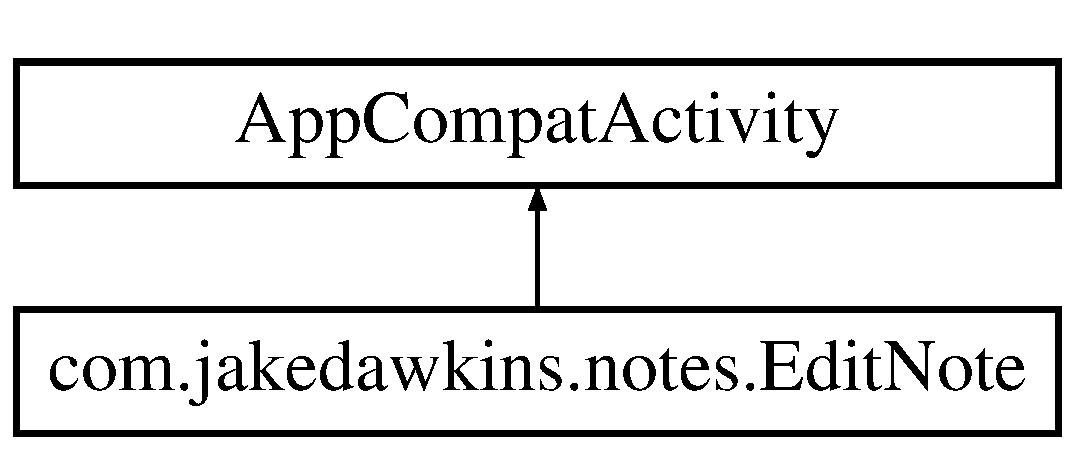
\includegraphics[height=2.000000cm]{classcom_1_1jakedawkins_1_1notes_1_1_edit_note}
\end{center}
\end{figure}
\subsection*{Public Member Functions}
\begin{DoxyCompactItemize}
\item 
void \hyperlink{classcom_1_1jakedawkins_1_1notes_1_1_edit_note_aaef5d6143b3e91e3581f1c886f574c34}{save\+Note} (View view)
\item 
void \hyperlink{classcom_1_1jakedawkins_1_1notes_1_1_edit_note_a12e30301cd0b67c7b7537cd503664f68}{delete\+Note} (View view)
\end{DoxyCompactItemize}
\subsection*{Protected Member Functions}
\begin{DoxyCompactItemize}
\item 
void \hyperlink{classcom_1_1jakedawkins_1_1notes_1_1_edit_note_a5cef19abb2116a93f1b72828ae098db4}{on\+Create} (Bundle saved\+Instance\+State)
\end{DoxyCompactItemize}


\subsection{Member Function Documentation}
\index{com\+::jakedawkins\+::notes\+::\+Edit\+Note@{com\+::jakedawkins\+::notes\+::\+Edit\+Note}!delete\+Note@{delete\+Note}}
\index{delete\+Note@{delete\+Note}!com\+::jakedawkins\+::notes\+::\+Edit\+Note@{com\+::jakedawkins\+::notes\+::\+Edit\+Note}}
\subsubsection[{\texorpdfstring{delete\+Note(\+View view)}{deleteNote(View view)}}]{\setlength{\rightskip}{0pt plus 5cm}void com.\+jakedawkins.\+notes.\+Edit\+Note.\+delete\+Note (
\begin{DoxyParamCaption}
\item[{View}]{view}
\end{DoxyParamCaption}
)}\hypertarget{classcom_1_1jakedawkins_1_1notes_1_1_edit_note_a12e30301cd0b67c7b7537cd503664f68}{}\label{classcom_1_1jakedawkins_1_1notes_1_1_edit_note_a12e30301cd0b67c7b7537cd503664f68}
takes an already existing note and removes it from List and DB


\begin{DoxyParams}{Parameters}
{\em View} & $\vert$ button pressed \\
\hline
\end{DoxyParams}
\index{com\+::jakedawkins\+::notes\+::\+Edit\+Note@{com\+::jakedawkins\+::notes\+::\+Edit\+Note}!on\+Create@{on\+Create}}
\index{on\+Create@{on\+Create}!com\+::jakedawkins\+::notes\+::\+Edit\+Note@{com\+::jakedawkins\+::notes\+::\+Edit\+Note}}
\subsubsection[{\texorpdfstring{on\+Create(\+Bundle saved\+Instance\+State)}{onCreate(Bundle savedInstanceState)}}]{\setlength{\rightskip}{0pt plus 5cm}void com.\+jakedawkins.\+notes.\+Edit\+Note.\+on\+Create (
\begin{DoxyParamCaption}
\item[{Bundle}]{saved\+Instance\+State}
\end{DoxyParamCaption}
)\hspace{0.3cm}{\ttfamily [protected]}}\hypertarget{classcom_1_1jakedawkins_1_1notes_1_1_edit_note_a5cef19abb2116a93f1b72828ae098db4}{}\label{classcom_1_1jakedawkins_1_1notes_1_1_edit_note_a5cef19abb2116a93f1b72828ae098db4}
Get a support Action\+Bar corresponding to this toolbar

Enable the Up button

set up the textfields \index{com\+::jakedawkins\+::notes\+::\+Edit\+Note@{com\+::jakedawkins\+::notes\+::\+Edit\+Note}!save\+Note@{save\+Note}}
\index{save\+Note@{save\+Note}!com\+::jakedawkins\+::notes\+::\+Edit\+Note@{com\+::jakedawkins\+::notes\+::\+Edit\+Note}}
\subsubsection[{\texorpdfstring{save\+Note(\+View view)}{saveNote(View view)}}]{\setlength{\rightskip}{0pt plus 5cm}void com.\+jakedawkins.\+notes.\+Edit\+Note.\+save\+Note (
\begin{DoxyParamCaption}
\item[{View}]{view}
\end{DoxyParamCaption}
)}\hypertarget{classcom_1_1jakedawkins_1_1notes_1_1_edit_note_aaef5d6143b3e91e3581f1c886f574c34}{}\label{classcom_1_1jakedawkins_1_1notes_1_1_edit_note_aaef5d6143b3e91e3581f1c886f574c34}
takes an already existing note and saves it.


\begin{DoxyParams}{Parameters}
{\em View} & $\vert$ button clicked \\
\hline
\end{DoxyParams}
set tags

let user know not all tags were valid 

The documentation for this class was generated from the following file\+:\begin{DoxyCompactItemize}
\item 
/\+Users/\+Jake/git/school/4820\+\_\+\+Android/jacksod.\+a2/\+Notes/app/src/main/java/com/jakedawkins/notes/Edit\+Note.\+java\end{DoxyCompactItemize}

\hypertarget{classcom_1_1jakedawkins_1_1notes_1_1_info_activity}{}\section{com.\+jakedawkins.\+notes.\+Info\+Activity Class Reference}
\label{classcom_1_1jakedawkins_1_1notes_1_1_info_activity}\index{com.\+jakedawkins.\+notes.\+Info\+Activity@{com.\+jakedawkins.\+notes.\+Info\+Activity}}
Inheritance diagram for com.\+jakedawkins.\+notes.\+Info\+Activity\+:\begin{figure}[H]
\begin{center}
\leavevmode
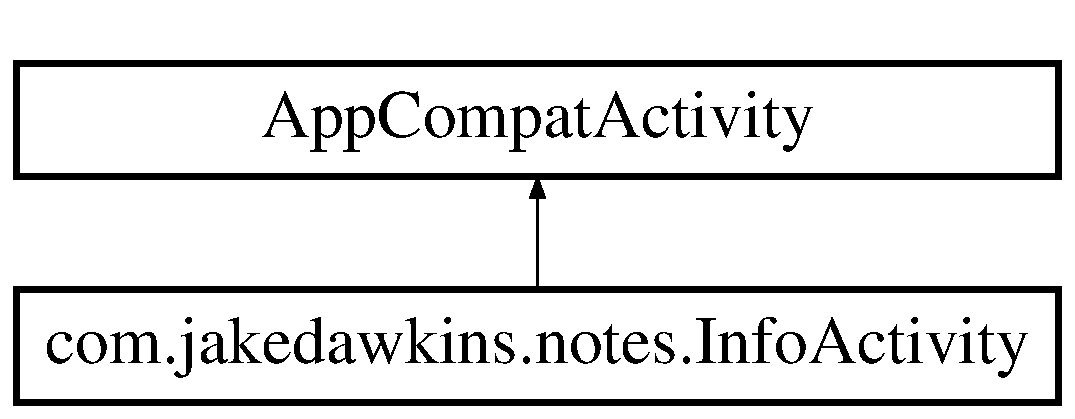
\includegraphics[height=2.000000cm]{classcom_1_1jakedawkins_1_1notes_1_1_info_activity}
\end{center}
\end{figure}
\subsection*{Protected Member Functions}
\begin{DoxyCompactItemize}
\item 
void \hyperlink{classcom_1_1jakedawkins_1_1notes_1_1_info_activity_a1c09d6ea23e38c19fa5bed0f1186d614}{on\+Create} (Bundle saved\+Instance\+State)
\end{DoxyCompactItemize}


\subsection{Member Function Documentation}
\index{com\+::jakedawkins\+::notes\+::\+Info\+Activity@{com\+::jakedawkins\+::notes\+::\+Info\+Activity}!on\+Create@{on\+Create}}
\index{on\+Create@{on\+Create}!com\+::jakedawkins\+::notes\+::\+Info\+Activity@{com\+::jakedawkins\+::notes\+::\+Info\+Activity}}
\subsubsection[{\texorpdfstring{on\+Create(\+Bundle saved\+Instance\+State)}{onCreate(Bundle savedInstanceState)}}]{\setlength{\rightskip}{0pt plus 5cm}void com.\+jakedawkins.\+notes.\+Info\+Activity.\+on\+Create (
\begin{DoxyParamCaption}
\item[{Bundle}]{saved\+Instance\+State}
\end{DoxyParamCaption}
)\hspace{0.3cm}{\ttfamily [protected]}}\hypertarget{classcom_1_1jakedawkins_1_1notes_1_1_info_activity_a1c09d6ea23e38c19fa5bed0f1186d614}{}\label{classcom_1_1jakedawkins_1_1notes_1_1_info_activity_a1c09d6ea23e38c19fa5bed0f1186d614}
Get a support Action\+Bar corresponding to this toolbar

Enable the Up button 

The documentation for this class was generated from the following file\+:\begin{DoxyCompactItemize}
\item 
/\+Users/\+Jake/git/school/4820\+\_\+\+Android/jacksod.\+a2/\+Notes/app/src/main/java/com/jakedawkins/notes/Info\+Activity.\+java\end{DoxyCompactItemize}

\hypertarget{classcom_1_1jakedawkins_1_1notes_1_1_list_notes}{}\section{com.\+jakedawkins.\+notes.\+List\+Notes Class Reference}
\label{classcom_1_1jakedawkins_1_1notes_1_1_list_notes}\index{com.\+jakedawkins.\+notes.\+List\+Notes@{com.\+jakedawkins.\+notes.\+List\+Notes}}
Inheritance diagram for com.\+jakedawkins.\+notes.\+List\+Notes\+:\begin{figure}[H]
\begin{center}
\leavevmode
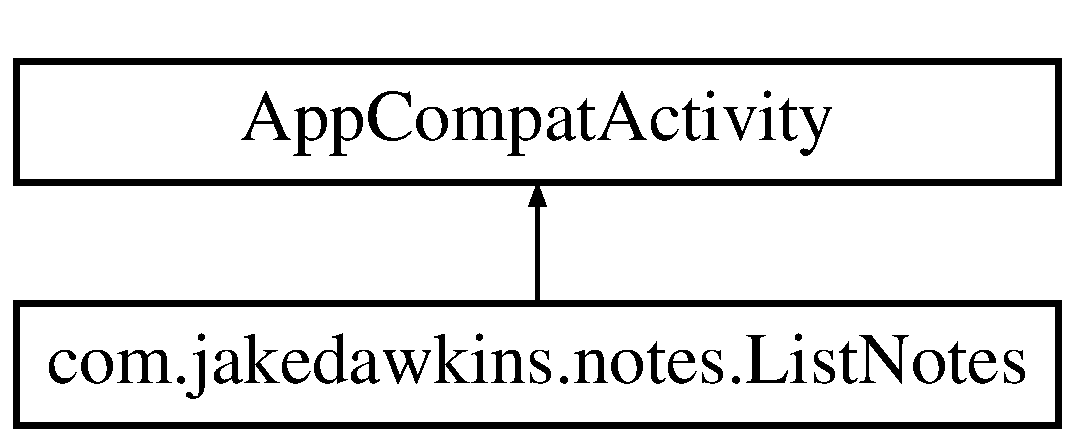
\includegraphics[height=2.000000cm]{classcom_1_1jakedawkins_1_1notes_1_1_list_notes}
\end{center}
\end{figure}
\subsection*{Public Member Functions}
\begin{DoxyCompactItemize}
\item 
void \hyperlink{classcom_1_1jakedawkins_1_1notes_1_1_list_notes_a18e83462a551ec45bde3a6040267fdc8}{new\+Note} (View view)
\item 
boolean \hyperlink{classcom_1_1jakedawkins_1_1notes_1_1_list_notes_a6b4df66f8083efa67bae77294b2c6a6b}{to\+Info\+Activity} (Menu\+Item item)
\item 
boolean \hyperlink{classcom_1_1jakedawkins_1_1notes_1_1_list_notes_ac97485ae407d36a55b0c2994bbaaa228}{on\+Create\+Options\+Menu} (Menu menu)
\item 
void \hyperlink{classcom_1_1jakedawkins_1_1notes_1_1_list_notes_a78c2ab7f4a94ab8efbe36b1c9be81b60}{on\+Resume} ()
\end{DoxyCompactItemize}
\subsection*{Protected Member Functions}
\begin{DoxyCompactItemize}
\item 
void \hyperlink{classcom_1_1jakedawkins_1_1notes_1_1_list_notes_a39a41b19881da4d8ac90ac3bacbf95a1}{on\+Create} (Bundle saved\+Instance\+State)
\end{DoxyCompactItemize}


\subsection{Member Function Documentation}
\index{com\+::jakedawkins\+::notes\+::\+List\+Notes@{com\+::jakedawkins\+::notes\+::\+List\+Notes}!new\+Note@{new\+Note}}
\index{new\+Note@{new\+Note}!com\+::jakedawkins\+::notes\+::\+List\+Notes@{com\+::jakedawkins\+::notes\+::\+List\+Notes}}
\subsubsection[{\texorpdfstring{new\+Note(\+View view)}{newNote(View view)}}]{\setlength{\rightskip}{0pt plus 5cm}void com.\+jakedawkins.\+notes.\+List\+Notes.\+new\+Note (
\begin{DoxyParamCaption}
\item[{View}]{view}
\end{DoxyParamCaption}
)}\hypertarget{classcom_1_1jakedawkins_1_1notes_1_1_list_notes_a18e83462a551ec45bde3a6040267fdc8}{}\label{classcom_1_1jakedawkins_1_1notes_1_1_list_notes_a18e83462a551ec45bde3a6040267fdc8}
Launches a new activity for creating a new note


\begin{DoxyParams}{Parameters}
{\em view$\vert$} & button clicked \\
\hline
\end{DoxyParams}
\index{com\+::jakedawkins\+::notes\+::\+List\+Notes@{com\+::jakedawkins\+::notes\+::\+List\+Notes}!on\+Create@{on\+Create}}
\index{on\+Create@{on\+Create}!com\+::jakedawkins\+::notes\+::\+List\+Notes@{com\+::jakedawkins\+::notes\+::\+List\+Notes}}
\subsubsection[{\texorpdfstring{on\+Create(\+Bundle saved\+Instance\+State)}{onCreate(Bundle savedInstanceState)}}]{\setlength{\rightskip}{0pt plus 5cm}void com.\+jakedawkins.\+notes.\+List\+Notes.\+on\+Create (
\begin{DoxyParamCaption}
\item[{Bundle}]{saved\+Instance\+State}
\end{DoxyParamCaption}
)\hspace{0.3cm}{\ttfamily [protected]}}\hypertarget{classcom_1_1jakedawkins_1_1notes_1_1_list_notes_a39a41b19881da4d8ac90ac3bacbf95a1}{}\label{classcom_1_1jakedawkins_1_1notes_1_1_list_notes_a39a41b19881da4d8ac90ac3bacbf95a1}
load up the db and retrieve notes

fill notes table

set up note adapter

link adapter to list\+View \index{com\+::jakedawkins\+::notes\+::\+List\+Notes@{com\+::jakedawkins\+::notes\+::\+List\+Notes}!on\+Create\+Options\+Menu@{on\+Create\+Options\+Menu}}
\index{on\+Create\+Options\+Menu@{on\+Create\+Options\+Menu}!com\+::jakedawkins\+::notes\+::\+List\+Notes@{com\+::jakedawkins\+::notes\+::\+List\+Notes}}
\subsubsection[{\texorpdfstring{on\+Create\+Options\+Menu(\+Menu menu)}{onCreateOptionsMenu(Menu menu)}}]{\setlength{\rightskip}{0pt plus 5cm}boolean com.\+jakedawkins.\+notes.\+List\+Notes.\+on\+Create\+Options\+Menu (
\begin{DoxyParamCaption}
\item[{Menu}]{menu}
\end{DoxyParamCaption}
)}\hypertarget{classcom_1_1jakedawkins_1_1notes_1_1_list_notes_ac97485ae407d36a55b0c2994bbaaa228}{}\label{classcom_1_1jakedawkins_1_1notes_1_1_list_notes_ac97485ae407d36a55b0c2994bbaaa228}
Inflate the menu; this adds items to the action bar if it is present. \index{com\+::jakedawkins\+::notes\+::\+List\+Notes@{com\+::jakedawkins\+::notes\+::\+List\+Notes}!on\+Resume@{on\+Resume}}
\index{on\+Resume@{on\+Resume}!com\+::jakedawkins\+::notes\+::\+List\+Notes@{com\+::jakedawkins\+::notes\+::\+List\+Notes}}
\subsubsection[{\texorpdfstring{on\+Resume()}{onResume()}}]{\setlength{\rightskip}{0pt plus 5cm}void com.\+jakedawkins.\+notes.\+List\+Notes.\+on\+Resume (
\begin{DoxyParamCaption}
{}
\end{DoxyParamCaption}
)}\hypertarget{classcom_1_1jakedawkins_1_1notes_1_1_list_notes_a78c2ab7f4a94ab8efbe36b1c9be81b60}{}\label{classcom_1_1jakedawkins_1_1notes_1_1_list_notes_a78c2ab7f4a94ab8efbe36b1c9be81b60}
gets called whenever a user leaves the view (to another app/view) \index{com\+::jakedawkins\+::notes\+::\+List\+Notes@{com\+::jakedawkins\+::notes\+::\+List\+Notes}!to\+Info\+Activity@{to\+Info\+Activity}}
\index{to\+Info\+Activity@{to\+Info\+Activity}!com\+::jakedawkins\+::notes\+::\+List\+Notes@{com\+::jakedawkins\+::notes\+::\+List\+Notes}}
\subsubsection[{\texorpdfstring{to\+Info\+Activity(\+Menu\+Item item)}{toInfoActivity(MenuItem item)}}]{\setlength{\rightskip}{0pt plus 5cm}boolean com.\+jakedawkins.\+notes.\+List\+Notes.\+to\+Info\+Activity (
\begin{DoxyParamCaption}
\item[{Menu\+Item}]{item}
\end{DoxyParamCaption}
)}\hypertarget{classcom_1_1jakedawkins_1_1notes_1_1_list_notes_a6b4df66f8083efa67bae77294b2c6a6b}{}\label{classcom_1_1jakedawkins_1_1notes_1_1_list_notes_a6b4df66f8083efa67bae77294b2c6a6b}
Launches a new activity for viewing information


\begin{DoxyParams}{Parameters}
{\em item$\vert$} & button clicked \\
\hline
\end{DoxyParams}


The documentation for this class was generated from the following file\+:\begin{DoxyCompactItemize}
\item 
/\+Users/\+Jake/git/school/4820\+\_\+\+Android/jacksod.\+a2/\+Notes/app/src/main/java/com/jakedawkins/notes/List\+Notes.\+java\end{DoxyCompactItemize}

\hypertarget{classcom_1_1jakedawkins_1_1notes_1_1_new_note}{}\section{com.\+jakedawkins.\+notes.\+New\+Note Class Reference}
\label{classcom_1_1jakedawkins_1_1notes_1_1_new_note}\index{com.\+jakedawkins.\+notes.\+New\+Note@{com.\+jakedawkins.\+notes.\+New\+Note}}
Inheritance diagram for com.\+jakedawkins.\+notes.\+New\+Note\+:\begin{figure}[H]
\begin{center}
\leavevmode
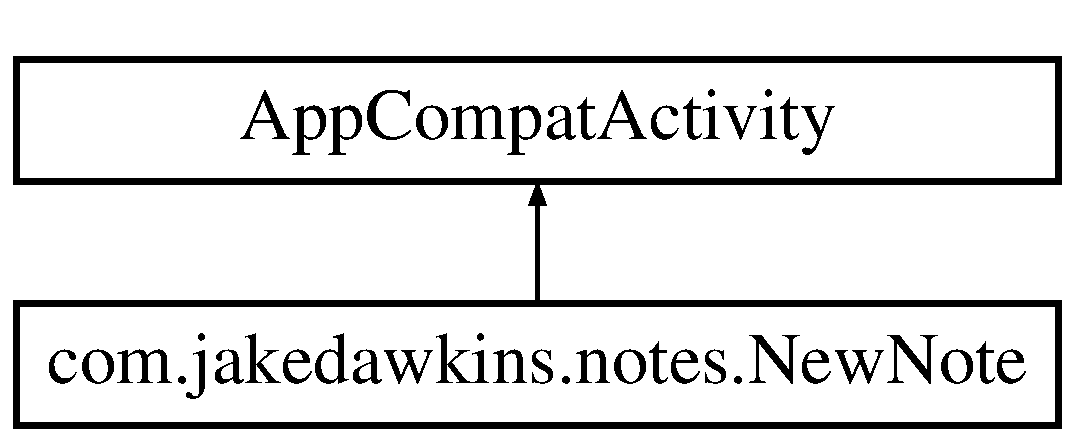
\includegraphics[height=2.000000cm]{classcom_1_1jakedawkins_1_1notes_1_1_new_note}
\end{center}
\end{figure}
\subsection*{Public Member Functions}
\begin{DoxyCompactItemize}
\item 
void \hyperlink{classcom_1_1jakedawkins_1_1notes_1_1_new_note_ab67e5f45d753178431b8f30bf027b63a}{save\+Note} (View view)
\item 
void \hyperlink{classcom_1_1jakedawkins_1_1notes_1_1_new_note_a18447103f8d0ad6611cb1fc082cd28b0}{new\+Photo} (View view)\hypertarget{classcom_1_1jakedawkins_1_1notes_1_1_new_note_a18447103f8d0ad6611cb1fc082cd28b0}{}\label{classcom_1_1jakedawkins_1_1notes_1_1_new_note_a18447103f8d0ad6611cb1fc082cd28b0}

\begin{DoxyCompactList}\small\item\em user presses add photo button \end{DoxyCompactList}\item 
void \hyperlink{classcom_1_1jakedawkins_1_1notes_1_1_new_note_ad92ba94cc2ee93cf75608fb418e8fffd}{remove\+Photo} (View view)\hypertarget{classcom_1_1jakedawkins_1_1notes_1_1_new_note_ad92ba94cc2ee93cf75608fb418e8fffd}{}\label{classcom_1_1jakedawkins_1_1notes_1_1_new_note_ad92ba94cc2ee93cf75608fb418e8fffd}

\begin{DoxyCompactList}\small\item\em removes the photo from the note \end{DoxyCompactList}\end{DoxyCompactItemize}
\subsection*{Protected Member Functions}
\begin{DoxyCompactItemize}
\item 
void \hyperlink{classcom_1_1jakedawkins_1_1notes_1_1_new_note_a833d4ae579733d1218d8fc84f0f44ba0}{on\+Create} (Bundle saved\+Instance\+State)
\item 
void \hyperlink{classcom_1_1jakedawkins_1_1notes_1_1_new_note_a458daf0172da2b7a7357e93dd4837179}{on\+Activity\+Result} (int request\+Code, int result\+Code, Intent data)\hypertarget{classcom_1_1jakedawkins_1_1notes_1_1_new_note_a458daf0172da2b7a7357e93dd4837179}{}\label{classcom_1_1jakedawkins_1_1notes_1_1_new_note_a458daf0172da2b7a7357e93dd4837179}

\begin{DoxyCompactList}\small\item\em after the image picker returns \end{DoxyCompactList}\end{DoxyCompactItemize}


\subsection{Member Function Documentation}
\index{com\+::jakedawkins\+::notes\+::\+New\+Note@{com\+::jakedawkins\+::notes\+::\+New\+Note}!on\+Create@{on\+Create}}
\index{on\+Create@{on\+Create}!com\+::jakedawkins\+::notes\+::\+New\+Note@{com\+::jakedawkins\+::notes\+::\+New\+Note}}
\subsubsection[{\texorpdfstring{on\+Create(\+Bundle saved\+Instance\+State)}{onCreate(Bundle savedInstanceState)}}]{\setlength{\rightskip}{0pt plus 5cm}void com.\+jakedawkins.\+notes.\+New\+Note.\+on\+Create (
\begin{DoxyParamCaption}
\item[{Bundle}]{saved\+Instance\+State}
\end{DoxyParamCaption}
)\hspace{0.3cm}{\ttfamily [inline]}, {\ttfamily [protected]}}\hypertarget{classcom_1_1jakedawkins_1_1notes_1_1_new_note_a833d4ae579733d1218d8fc84f0f44ba0}{}\label{classcom_1_1jakedawkins_1_1notes_1_1_new_note_a833d4ae579733d1218d8fc84f0f44ba0}
Get a support Action\+Bar corresponding to this toolbar

Enable the Up button

hide the image/button layout \index{com\+::jakedawkins\+::notes\+::\+New\+Note@{com\+::jakedawkins\+::notes\+::\+New\+Note}!save\+Note@{save\+Note}}
\index{save\+Note@{save\+Note}!com\+::jakedawkins\+::notes\+::\+New\+Note@{com\+::jakedawkins\+::notes\+::\+New\+Note}}
\subsubsection[{\texorpdfstring{save\+Note(\+View view)}{saveNote(View view)}}]{\setlength{\rightskip}{0pt plus 5cm}void com.\+jakedawkins.\+notes.\+New\+Note.\+save\+Note (
\begin{DoxyParamCaption}
\item[{View}]{view}
\end{DoxyParamCaption}
)\hspace{0.3cm}{\ttfamily [inline]}}\hypertarget{classcom_1_1jakedawkins_1_1notes_1_1_new_note_ab67e5f45d753178431b8f30bf027b63a}{}\label{classcom_1_1jakedawkins_1_1notes_1_1_new_note_ab67e5f45d753178431b8f30bf027b63a}
takes a new note and saves it to the list and DB


\begin{DoxyParams}{Parameters}
{\em View} & $\vert$ button pressed \\
\hline
\end{DoxyParams}
set tags

let user know not all tags were valid

add the image bitmap to the note for saving

return back to the previous activity 

The documentation for this class was generated from the following file\+:\begin{DoxyCompactItemize}
\item 
/\+Users/jake/git/school/4820\+\_\+\+Android/jacksod.\+a3/\+Notes/app/src/main/java/com/jakedawkins/notes/New\+Note.\+java\end{DoxyCompactItemize}

\hypertarget{classcom_1_1jakedawkins_1_1notes_1_1_note}{}\section{com.\+jakedawkins.\+notes.\+Note Class Reference}
\label{classcom_1_1jakedawkins_1_1notes_1_1_note}\index{com.\+jakedawkins.\+notes.\+Note@{com.\+jakedawkins.\+notes.\+Note}}
\subsection*{Public Member Functions}
\begin{DoxyCompactItemize}
\item 
void {\bfseries set\+ID} (int id)\hypertarget{classcom_1_1jakedawkins_1_1notes_1_1_note_a876432b6d8ebdefe19913e56e25a7f55}{}\label{classcom_1_1jakedawkins_1_1notes_1_1_note_a876432b6d8ebdefe19913e56e25a7f55}

\item 
void {\bfseries set\+Text} (String text)\hypertarget{classcom_1_1jakedawkins_1_1notes_1_1_note_ac1e2f35722960be015d567988bee7ae8}{}\label{classcom_1_1jakedawkins_1_1notes_1_1_note_ac1e2f35722960be015d567988bee7ae8}

\item 
void {\bfseries set\+Created} (String created)\hypertarget{classcom_1_1jakedawkins_1_1notes_1_1_note_a09b6be123b9c33bc1232bb2f3fd095c3}{}\label{classcom_1_1jakedawkins_1_1notes_1_1_note_a09b6be123b9c33bc1232bb2f3fd095c3}

\item 
void \hyperlink{classcom_1_1jakedawkins_1_1notes_1_1_note_a3c1aa05b41c222b6225c4c17c27f2b6a}{create\+Now} ()
\item 
void {\bfseries set\+Updated} (String updated)\hypertarget{classcom_1_1jakedawkins_1_1notes_1_1_note_a64f269e798088cfbcd478706b740e876}{}\label{classcom_1_1jakedawkins_1_1notes_1_1_note_a64f269e798088cfbcd478706b740e876}

\item 
void \hyperlink{classcom_1_1jakedawkins_1_1notes_1_1_note_a244c89c05ab7d2664d648cf111ae994c}{update\+Now} ()
\item 
String {\bfseries get\+Text} ()\hypertarget{classcom_1_1jakedawkins_1_1notes_1_1_note_aa55302a567a3c1b0474bba551f5f1862}{}\label{classcom_1_1jakedawkins_1_1notes_1_1_note_aa55302a567a3c1b0474bba551f5f1862}

\item 
int {\bfseries get\+ID} ()\hypertarget{classcom_1_1jakedawkins_1_1notes_1_1_note_a41d768d733d99d3c876441cc335bd47c}{}\label{classcom_1_1jakedawkins_1_1notes_1_1_note_a41d768d733d99d3c876441cc335bd47c}

\item 
String {\bfseries get\+Created} ()\hypertarget{classcom_1_1jakedawkins_1_1notes_1_1_note_ab44b461028520f61d280a993db893af0}{}\label{classcom_1_1jakedawkins_1_1notes_1_1_note_ab44b461028520f61d280a993db893af0}

\item 
String {\bfseries get\+Updated} ()\hypertarget{classcom_1_1jakedawkins_1_1notes_1_1_note_a85712f0c56509074ceba01b7c39e7e05}{}\label{classcom_1_1jakedawkins_1_1notes_1_1_note_a85712f0c56509074ceba01b7c39e7e05}

\item 
Array\+List$<$ String $>$ \hyperlink{classcom_1_1jakedawkins_1_1notes_1_1_note_ac05c4f93746bcb3574560be52b9e12a4}{get\+Tags} ()
\item 
void \hyperlink{classcom_1_1jakedawkins_1_1notes_1_1_note_a24042a273e162d696ec882ec5b0a21c5}{add\+Tag} (String tag)
\item 
String \hyperlink{classcom_1_1jakedawkins_1_1notes_1_1_note_a313500b76d16857e2f8228dcba99231b}{tags\+To\+String} ()
\item 
String \hyperlink{classcom_1_1jakedawkins_1_1notes_1_1_note_aee327d73e1b9585ff5ad89faee39eb1a}{tags\+To\+Hashtags} ()
\item 
String \hyperlink{classcom_1_1jakedawkins_1_1notes_1_1_note_a66208950f8504449e3ce85e3a1b82c8f}{now} ()
\end{DoxyCompactItemize}


\subsection{Detailed Description}
\hyperlink{classcom_1_1jakedawkins_1_1notes_1_1_note}{Note} class containing all basic info for a note including a helper to set the timedate for updated/created to now 

\subsection{Member Function Documentation}
\index{com\+::jakedawkins\+::notes\+::\+Note@{com\+::jakedawkins\+::notes\+::\+Note}!add\+Tag@{add\+Tag}}
\index{add\+Tag@{add\+Tag}!com\+::jakedawkins\+::notes\+::\+Note@{com\+::jakedawkins\+::notes\+::\+Note}}
\subsubsection[{\texorpdfstring{add\+Tag(\+String tag)}{addTag(String tag)}}]{\setlength{\rightskip}{0pt plus 5cm}void com.\+jakedawkins.\+notes.\+Note.\+add\+Tag (
\begin{DoxyParamCaption}
\item[{String}]{tag}
\end{DoxyParamCaption}
)}\hypertarget{classcom_1_1jakedawkins_1_1notes_1_1_note_a24042a273e162d696ec882ec5b0a21c5}{}\label{classcom_1_1jakedawkins_1_1notes_1_1_note_a24042a273e162d696ec882ec5b0a21c5}
assumes tag has already been checked for validity (alphanumeric or \+\_\+)


\begin{DoxyParams}{Parameters}
{\em tag$\vert$} & string of new taf to add \\
\hline
\end{DoxyParams}
\index{com\+::jakedawkins\+::notes\+::\+Note@{com\+::jakedawkins\+::notes\+::\+Note}!create\+Now@{create\+Now}}
\index{create\+Now@{create\+Now}!com\+::jakedawkins\+::notes\+::\+Note@{com\+::jakedawkins\+::notes\+::\+Note}}
\subsubsection[{\texorpdfstring{create\+Now()}{createNow()}}]{\setlength{\rightskip}{0pt plus 5cm}void com.\+jakedawkins.\+notes.\+Note.\+create\+Now (
\begin{DoxyParamCaption}
{}
\end{DoxyParamCaption}
)}\hypertarget{classcom_1_1jakedawkins_1_1notes_1_1_note_a3c1aa05b41c222b6225c4c17c27f2b6a}{}\label{classcom_1_1jakedawkins_1_1notes_1_1_note_a3c1aa05b41c222b6225c4c17c27f2b6a}
Sets the created Time\+Date to the current Time\+Date \index{com\+::jakedawkins\+::notes\+::\+Note@{com\+::jakedawkins\+::notes\+::\+Note}!get\+Tags@{get\+Tags}}
\index{get\+Tags@{get\+Tags}!com\+::jakedawkins\+::notes\+::\+Note@{com\+::jakedawkins\+::notes\+::\+Note}}
\subsubsection[{\texorpdfstring{get\+Tags()}{getTags()}}]{\setlength{\rightskip}{0pt plus 5cm}Array\+List$<$String$>$ com.\+jakedawkins.\+notes.\+Note.\+get\+Tags (
\begin{DoxyParamCaption}
{}
\end{DoxyParamCaption}
)}\hypertarget{classcom_1_1jakedawkins_1_1notes_1_1_note_ac05c4f93746bcb3574560be52b9e12a4}{}\label{classcom_1_1jakedawkins_1_1notes_1_1_note_ac05c4f93746bcb3574560be52b9e12a4}
\begin{DoxyReturn}{Returns}
Array\+List$<$\+String$>$$\vert$ list of all the tags associated with the note 
\end{DoxyReturn}
\index{com\+::jakedawkins\+::notes\+::\+Note@{com\+::jakedawkins\+::notes\+::\+Note}!now@{now}}
\index{now@{now}!com\+::jakedawkins\+::notes\+::\+Note@{com\+::jakedawkins\+::notes\+::\+Note}}
\subsubsection[{\texorpdfstring{now()}{now()}}]{\setlength{\rightskip}{0pt plus 5cm}String com.\+jakedawkins.\+notes.\+Note.\+now (
\begin{DoxyParamCaption}
{}
\end{DoxyParamCaption}
)}\hypertarget{classcom_1_1jakedawkins_1_1notes_1_1_note_a66208950f8504449e3ce85e3a1b82c8f}{}\label{classcom_1_1jakedawkins_1_1notes_1_1_note_a66208950f8504449e3ce85e3a1b82c8f}
Used to generate a my\+S\+Q\+L-\/like timedate string of right now in format of Y\+Y\+Y\+Y-\/\+M\+M-\/\+DD H\+H\+:\+MM\+:SS

\begin{DoxyReturn}{Returns}
String$\vert$ current time\+Date string 
\end{DoxyReturn}
\index{com\+::jakedawkins\+::notes\+::\+Note@{com\+::jakedawkins\+::notes\+::\+Note}!tags\+To\+Hashtags@{tags\+To\+Hashtags}}
\index{tags\+To\+Hashtags@{tags\+To\+Hashtags}!com\+::jakedawkins\+::notes\+::\+Note@{com\+::jakedawkins\+::notes\+::\+Note}}
\subsubsection[{\texorpdfstring{tags\+To\+Hashtags()}{tagsToHashtags()}}]{\setlength{\rightskip}{0pt plus 5cm}String com.\+jakedawkins.\+notes.\+Note.\+tags\+To\+Hashtags (
\begin{DoxyParamCaption}
{}
\end{DoxyParamCaption}
)}\hypertarget{classcom_1_1jakedawkins_1_1notes_1_1_note_aee327d73e1b9585ff5ad89faee39eb1a}{}\label{classcom_1_1jakedawkins_1_1notes_1_1_note_aee327d73e1b9585ff5ad89faee39eb1a}
Used to generate a list of tags, prefixed with a pound sign (hashtag), that can be displayed as a single string

\begin{DoxyReturn}{Returns}
String$\vert$ list of tags in plaintext 
\end{DoxyReturn}
\index{com\+::jakedawkins\+::notes\+::\+Note@{com\+::jakedawkins\+::notes\+::\+Note}!tags\+To\+String@{tags\+To\+String}}
\index{tags\+To\+String@{tags\+To\+String}!com\+::jakedawkins\+::notes\+::\+Note@{com\+::jakedawkins\+::notes\+::\+Note}}
\subsubsection[{\texorpdfstring{tags\+To\+String()}{tagsToString()}}]{\setlength{\rightskip}{0pt plus 5cm}String com.\+jakedawkins.\+notes.\+Note.\+tags\+To\+String (
\begin{DoxyParamCaption}
{}
\end{DoxyParamCaption}
)}\hypertarget{classcom_1_1jakedawkins_1_1notes_1_1_note_a313500b76d16857e2f8228dcba99231b}{}\label{classcom_1_1jakedawkins_1_1notes_1_1_note_a313500b76d16857e2f8228dcba99231b}
Used to generate a list of tags that can be displayed as a single String

\begin{DoxyReturn}{Returns}
String$\vert$ list of tags in plaintext 
\end{DoxyReturn}
\index{com\+::jakedawkins\+::notes\+::\+Note@{com\+::jakedawkins\+::notes\+::\+Note}!update\+Now@{update\+Now}}
\index{update\+Now@{update\+Now}!com\+::jakedawkins\+::notes\+::\+Note@{com\+::jakedawkins\+::notes\+::\+Note}}
\subsubsection[{\texorpdfstring{update\+Now()}{updateNow()}}]{\setlength{\rightskip}{0pt plus 5cm}void com.\+jakedawkins.\+notes.\+Note.\+update\+Now (
\begin{DoxyParamCaption}
{}
\end{DoxyParamCaption}
)}\hypertarget{classcom_1_1jakedawkins_1_1notes_1_1_note_a244c89c05ab7d2664d648cf111ae994c}{}\label{classcom_1_1jakedawkins_1_1notes_1_1_note_a244c89c05ab7d2664d648cf111ae994c}
Sets the updated Time\+Date to the current Time\+Date 

The documentation for this class was generated from the following file\+:\begin{DoxyCompactItemize}
\item 
/\+Users/\+Jake/git/school/4820\+\_\+\+Android/jacksod.\+a2/\+Notes/app/src/main/java/com/jakedawkins/notes/Note.\+java\end{DoxyCompactItemize}

\hypertarget{classcom_1_1jakedawkins_1_1notes_1_1_note_adapter}{}\section{com.\+jakedawkins.\+notes.\+Note\+Adapter Class Reference}
\label{classcom_1_1jakedawkins_1_1notes_1_1_note_adapter}\index{com.\+jakedawkins.\+notes.\+Note\+Adapter@{com.\+jakedawkins.\+notes.\+Note\+Adapter}}
Inheritance diagram for com.\+jakedawkins.\+notes.\+Note\+Adapter\+:\begin{figure}[H]
\begin{center}
\leavevmode
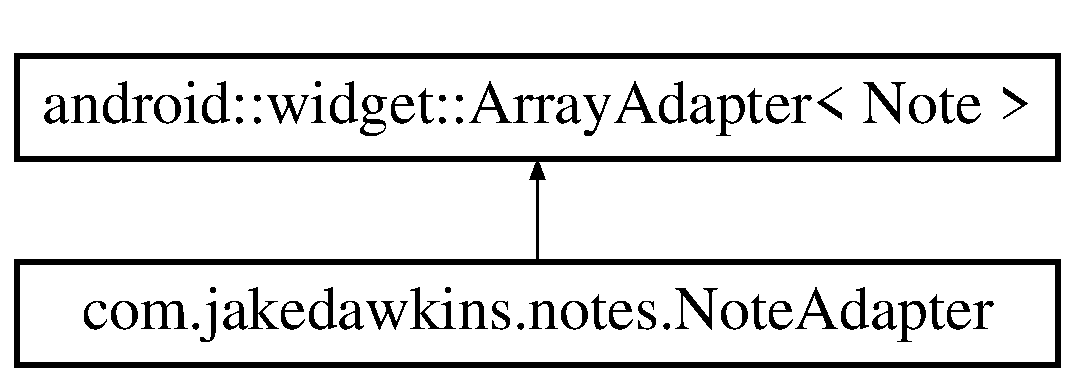
\includegraphics[height=2.000000cm]{classcom_1_1jakedawkins_1_1notes_1_1_note_adapter}
\end{center}
\end{figure}
\subsection*{Public Member Functions}
\begin{DoxyCompactItemize}
\item 
{\bfseries Note\+Adapter} (Context context, Array\+List$<$ \hyperlink{classcom_1_1jakedawkins_1_1notes_1_1_note}{Note} $>$ notes)\hypertarget{classcom_1_1jakedawkins_1_1notes_1_1_note_adapter_a08bd80079044ffa1a2cedbc23af12e24}{}\label{classcom_1_1jakedawkins_1_1notes_1_1_note_adapter_a08bd80079044ffa1a2cedbc23af12e24}

\item 
View \hyperlink{classcom_1_1jakedawkins_1_1notes_1_1_note_adapter_a7a4ef147743422a5a87f93a1958b185f}{get\+View} (int position, View convert\+View, View\+Group parent)
\end{DoxyCompactItemize}


\subsection{Detailed Description}
Created by Jake on 2/1/16. 

\subsection{Member Function Documentation}
\index{com\+::jakedawkins\+::notes\+::\+Note\+Adapter@{com\+::jakedawkins\+::notes\+::\+Note\+Adapter}!get\+View@{get\+View}}
\index{get\+View@{get\+View}!com\+::jakedawkins\+::notes\+::\+Note\+Adapter@{com\+::jakedawkins\+::notes\+::\+Note\+Adapter}}
\subsubsection[{\texorpdfstring{get\+View(int position, View convert\+View, View\+Group parent)}{getView(int position, View convertView, ViewGroup parent)}}]{\setlength{\rightskip}{0pt plus 5cm}View com.\+jakedawkins.\+notes.\+Note\+Adapter.\+get\+View (
\begin{DoxyParamCaption}
\item[{int}]{position, }
\item[{View}]{convert\+View, }
\item[{View\+Group}]{parent}
\end{DoxyParamCaption}
)}\hypertarget{classcom_1_1jakedawkins_1_1notes_1_1_note_adapter_a7a4ef147743422a5a87f93a1958b185f}{}\label{classcom_1_1jakedawkins_1_1notes_1_1_note_adapter_a7a4ef147743422a5a87f93a1958b185f}
get data for view

Check if an existing view is being reused, otherwise inflate the view

Lookup view for data population

Populate the data into the template view using the data object

Return the completed view to render on screen 

The documentation for this class was generated from the following file\+:\begin{DoxyCompactItemize}
\item 
/\+Users/\+Jake/git/school/4820\+\_\+\+Android/jacksod.\+a2/\+Notes/app/src/main/java/com/jakedawkins/notes/Note\+Adapter.\+java\end{DoxyCompactItemize}

%--- End generated contents ---

% Index
\backmatter
\newpage
\phantomsection
\clearemptydoublepage
\addcontentsline{toc}{chapter}{Index}
\printindex

\end{document}
